\section{Méthode des moindres carrés}
\begin{enumerate}
  \setcounter{enumi}{2}
  \item \q{Ecrire une fonction }\il{S(X, Y)}\q{ qui prend en argument les données issues de la MMT et qui
          retourne un vecteur }\il{Som}\q{ dans lequel seront rangées les valeurs :}
        \[
          \begin{array}{ccccc}
            \il{Sxi}  & \il{Sxiyi2} & \il{Syi}  & \il{Sxi2yi} & \il{Sxiyi} \\\\
            \il{Sxi3} & \il{Sxi2}   & \il{Syi3} & \il{Syi2}   & \il{n}
          \end{array}
        \]
        \codeFromFile{section-03/q3.py}


        \bigskip

  \item \q{Ecrire une fonction }\il{cercle(X, Y)}\q{ qui prend en argument les données issues de la MMT et
          qui retourne }\il{Xc}\q{ et }\il{Yc}\q{ les coordonnées du centre du cercle et }\il{R}\q{ le rayon du
          cercle passant au mieux.}

        \codeFromFile{section-03/q4.py}

        \bigskip

  \item \q{Compléter le script de manière à afficher sur une même figure la position des points (cercle rouge) mesurés
          ainsi que le cercle qui passe au mieux (défini par la méthode des moindres carrés). Le rayon moyen sera
          affiché sur la figure.}


        \bigskip

        \begin{dinglist}{111}
          \item  On crée d'abord la fonction \il{traceCercle} permettant de créer une liste de coordonnées cartésiennes
          correspondant à celles d'un cercle :
          \codeFromFile{section-03/q5-1.py}

          \item Puis on exécute le script suivant pour afficher ce qui est demandé :
          \codeFromFile{section-03/q5-2.py}

          \item On obtient alors la figure suivante :
          \begin{center}
            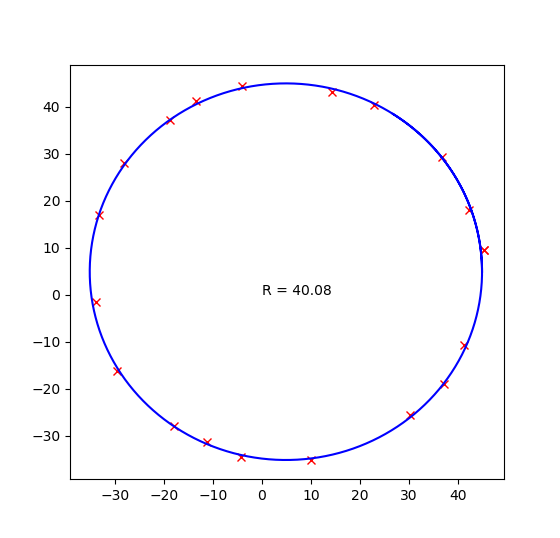
\includegraphics[scale=0.7]{section-03/q5-3.png}
          \end{center}
        \end{dinglist}

  \item \q{Ecrire une fonction }\il{circularite(Xc, Yc, R, X, Y)}\q{ prenant en argumant les paramètres du cercle 'qui
          passe au mieux' ainsi que les deux tableaux de coordonnées des points mesurés et qui retourne }\il{dc}\q{, le
          dédaut de circularité constaté ainsi que les distances des points les plus éloignés (}\il{Emax}\q{
          extérieurement, et }\il{Emin}\q{ intérieurement) au cercle $C$.}

        \codeFromFile{section-03/q6.py}


        \bigskip

  \item \q{Faire afficher sur le graphe précédent :}
        \begin{itemize}
          \item \q{$C_{max}$ concentrique à $C$ de diamètre le plus petit qui englobe tous les points $M_i$}
          \item \q{$C_{min}$ concentrique à $C$ de diamètre le plus grand qui ne contient aucun point $M_i$}
        \end{itemize}

        \bigskip

        \begin{dinglist}{111}
          \item On modifie le script précédent pour rajouter les cercles demandés :

          \bigskip

          \codeFromFile{section-03/q7-1.py}

          \bigskip

          \item Et on obtient la figure suivante :
          \begin{center}
            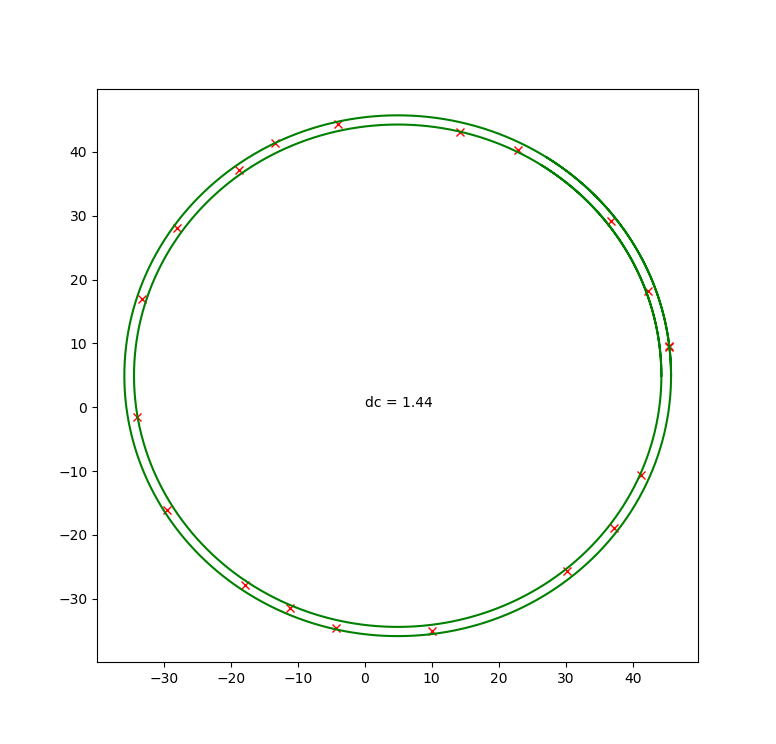
\includegraphics[scale=0.7]{section-03/q7-2.png}
          \end{center}
        \end{dinglist}
\end{enumerate}
